\chapter{Company to Symbol Linking}
\label{chap:comapny-to-symbol-linking}
This chapter delves into the challenge of linking companies mentioned in the text to their corresponding ticker symbols and exchanges. It highlights the limitations of the naive approach that relies on static data and score thresholds. However, it also introduces a more robust approach to entity linking using Wikidata. 

The cornerstone of the entity linking approach is the comprehensive Wikidata knowledge base. By leveraging structured data and relationships between entities, the entity linking method can effectively link companies to their ticker symbols, even if their names appear in different forms. Moreover, it eliminates the need for arbitrary score thresholds and provides access to wealthy company information.

The entity linking approach offers several advantages over the naive method, including increased accuracy, better handling of name variations, and access to comprehensive company data. However, it is crucial to recognize potential limitations. Nevertheless, the result shows that the entity linking approach using Wikidata is a powerful tool for linking companies to their ticker symbols, providing a flexible and accurate solution over the naive approach.\todo{TODO: Přidat nebo už je to moc navíc? The implementation involves using a spaCy entity linker pipeline built on a knowledge base to link text entities with Wikidata entities of the organization type. Subsequently, SPARQL queries are used to extract ticker symbols and exchanges from Wikidata, covering direct retrieval, owner-based retrieval, and differentiated retrieval scenarios.}

The chapter also distinguishes between a company and an organisation. A company certainly refers to an entity that trades on an exchange (has a ticker). In contrast, an organisation refers only to a potential candidate by named entity recognition that might be tradable on an exchange or associated with that company. In addition, the Python notebook\footnote{In the directory /ipynbs/company-to-symbol-linking/.} is provided for both sections of this chapter to guide the reader through the process by which the results were obtained.\todo{TODO: První část posledního odstavce pravděpodobně přesunu do Stock Exchange kapitoly, kde se budou popisovat nějaké základní info.}

\section{Introduction}
\label{sec:introduction}
Before proceeding further into this chapter, let us briefly revisit the concept of named entity recognition. It is a classification task to recognise entities within a given text, including names of organisations, people, places, dates, and more. While named entity recognition assigns entities to classes based on the syntax and semantics of the text, it does not provide specific details about individual entities. The necessity to identify companies in articles arises from their potential appearance in various forms and references. To give an example, the company Microsoft might be mentioned as ``\textit{Microsoft}'', ``\textit{Microsoft Corp.}'', ``\textit{Microsoft Corporation}'', or ``\textit{MSFT}''. In cases where multiple syntactic variations referring to the same company occur in an article, named entity recognition categorizes them all as organizations. However, it is crucial to have additional information to confirm that they represent the same entity. Bringing together these diverse forms\todo{TODO: Je nutná tato footnote?}\footnote{Different forms often encountered in newspaper articles due to authors' inconsistencies and text length.} into a single entity identifiable by a unique symbol is essential.

As discussed in the Stock Market\todo{TODO: Dodat odkaz a zmínit identifikátor v sekci.} section of Chapter \ref{chap:theoretical-background}, each company has a unique identifier called a ticker, used for stock market identification. This ticker must be assigned to every mention of the company within the article. Additionally, we need to ensure that every mention of a company has a corresponding ticker. The assignment facilitates the extraction of companies operating across various exchanges and helps eliminate unnecessary entities identified by named entity recognition. Not every organisation identified by named entity recognition, such as Greenpeace, the World Health Organization, or the United Nations, necessarily represents a company listed on the exchange. Moreover, this process will play a pivotal role in the subsequent stages of application development.

While some newspaper articles, such as those from Bloomberg, Reuters, and CNBC, may include a company's ticker symbol or another specific identifier immediately following its name in the text, as demonstrated by ``\textit{Microsoft (MSFT)}'', this practice is generally the exception rather than the norm across all news sources. Our primary textual data source, the Guardian, does not contain information about company tickers in this way (for more details, see Chapter \ref{chap:textual-data}). Hence, the task involves associating a company's name with its symbol. This chapter will focus on strategies for addressing this challenge, aiming to identify the optimal approach for handling this issue.

\section{Problem definition}
\label{sec:problem-definition}
Our objective is to address the challenge of assigning a unique identifier to each company mentioned in the text. Companies identified in the named entity recognition classification typically belong to the organisation class, narrowing our focus to entities categorised as organisations. In general, this challenge can be divided into three essential parts:

\begin{enumerate}
    \item[] \textbf{Input:} An article's text.
    \item[] \textbf{Output:} A set of companies with their unique identifiers.
    \item Recognising companies mentioned in the article.
    \item Assigning a unique identifier to each identified company, provided one exists.
    \item Extracting a set of companies contained in the article.
\end{enumerate}

The initial phase of the concern involves utilising named entity recognition to classify entities, as mentioned above, specifically focusing on those categorised as organisations. The subsequent step entails implementing a method to assign a unique identifier to each company. Hence, the second phase relies on matching company names against a database of companies and their detailed information. The third component is straightforward and involves the unification of all occurrences into a set of companies already assigned identifiers.

To ensure we take advantage of every mention of a company. In the subsequent sections, we will explore various methods that could address the given problem and select the most suitable one for our case. Let us consider the following excerpt from the article \parencite{TheGuardiaArticleDeepFake} about deepfake technology published by the Guardian on February 25, 2024:\begin{quote}
    \textit{``Executives from Adobe, Amazon, Google, IBM, Meta, Microsoft, OpenAI and TikTok gathered at the Munich Security Conference to announce a new framework for how they will respond to AI-generated deepfakes that deliberately trick voters.''}
\end{quote} The named entity recognition identifies Adobe, Amazon, Google, IBM, Microsoft, OpenAI, TikTok and Meta as organisations. It is good to note that TikTok is owned by ByteDance, not a publicly traded company. OpenAI finds itself in a similar position to that of a private company. Thus, buying directly from companies that own TikTok or OpenAI is impossible. However, a different scenario arises when discussing Facebook, Instagram, or Messenger, organisations owned by Meta, a publicly listed company on the exchange. The task is to assign the correct ticker symbol to each company mentioned in the article and to determine the stock exchange on which the company is listed. The following Table \ref{table:deepfake-article-excerpt} lists the companies mentioned in the article with their official name, corresponding ticker symbol, and stock exchange.

\begin{table}[ht]
    \centering
    \caption{Organisations identified in the Guardian's article about deepfake technology with their official names, ticker symbols, and stock exchanges.}
    \label{table:deepfake-article-excerpt}
    \begin{tabular}{l p{4cm} l l}
        \hline
        Organisation&Official Name&Ticker&Stock Exchange\\
        \hline
        Adobe&Adobe Inc.&ADBE&NASDAQ\\
        Amazon&Amazon.com Inc.&AMZN&NASDAQ\\
        Google&Alphabet Inc.&GOOGL&NASDAQ\\
        \multirow{2}{*}{IBM}&International Business Machines Corp.&\multirow{2}{*}{IBM}&\multirow{2}{*}{NYSE}\\
        Meta&Meta Platforms Inc.&META&NASDAQ\\        
        Microsoft&Microsoft Corp.&MSFT&NASDAQ\\
        OpenAI&N/A&N/A&N/A\\
        TikTok&N/A&N/A&N/A\\
        \hline
    \end{tabular}
\end{table}

According to Table \ref{table:deepfake-article-excerpt}, organisation names are not always identical to their official names. This prevalent discrepancy underscores the necessity to address this issue, which will be thoroughly examined in subsequent sections focusing on methods for linking company symbols. Consequently, our approach will leverage a database containing companies listed on exchanges and their corresponding tickers. This database will enable us to match the official names of companies with the recognised organisation entities extracted from the article. By obtaining the ticker symbol, we can confidently access additional information about the company from other databases, including its stock exchange listing and other pertinent details.

\section{Naive approach}
\label{sec:naive-approach}
Methods presented in this section are based on matching company names against an exchange static dataset of companies. The dataset contains a list of companies with their official name and ticker symbol. The naive approach involves comparing organisation names extracted from the article with the official names in the dataset. The corresponding ticker symbol and exchange are assigned to the organisation if a match is found. This straightforward approach is a good starting point for linking company names to their ticker symbols. However, it has its limitations, as it may not be able to handle variations in company names.

\subsection{Database}
\label{subsec:data-preparation}
The first step in implementing the naive approach is to obtain the data. We need a dataset containing company official names, ticker symbols, and information about relevant stock exchanges. The dataset should be in a format conducive to efficient processing, encompassing file formats such as CSV, JSON, and XML, or alternatively, be structured within a relational database table. We discovered suitable datasets of companies listed on various exchanges on the EODData website\footnote{\href{https://www.eoddata.com}{https://www.eoddata.com}}, with a particular focus on the NASDAQ, NYSE, and AMEX datasets. The datasets contain information about companies listed on exchanges, including their official names and ticker symbols. Each exchange has its dataset, so we have information on which exchange the company is listed. The datasets are in CSV format and can be easily preprocessed, allowing us to match organisation names extracted from the article.

\subsection{Data preprocessing}
\label{subsec:data-processing}
It would be beneficial to do some preprocessing before starting the matching process. This involves making a few simple adjustments to make it easier to compare individual strings. We execute these steps on the dataset of each exchange and the organisation names, which we are trying to match accurately. The preprocessing steps encompass:

\begin{description}
    \item[Lowercase conversion] Convert all characters to lowercase to ensure case-insensitive matching.
    \item[ASCII conversion] Convert all characters to ASCII to remove any non-ASCII characters in the string.
    \item[Punctuation removal] Remove punctuation to eliminate any special characters that could interfere with the matching process.
    \item[Common suffix removal] Remove common suffixes such as ``\textit{Inc.}'', ``\textit{Corp.}'', ``\textit{Ltd.}'', and similar terms, as their usage may be inconsistent across the article's company name and the dataset's official name.
    \item[Common word removal] Elimination of common words such as ``\textit{holding}'', ``\textit{company}'', ``\textit{group}'', and others, which may not be essential for matching the company name.
\end{description}

During the implementation, we discovered an effective Python library called Name Matching, available on GitHub\footnote{\href{https://www.github.com/DeNederlandscheBank/name\_matching/}{https://www.github.com/DeNederlandscheBank/name\_matching/}}. This library enables data preprocessing and the use of the distance metrics discussed in the following subsections. Additionally, after data preprocessing, the Cosine similarity method is used to reduce the number of potential matches by converting strings to n-grams and applying a \acrshort{tf-idf} transformation. With the preprocessed and reduced data in hand, we are ready to advance to the matching process based on distance metrics.\todo{Dopsat citace na cosine similarity a n-grams. + Ověřit správnost citace knihovny, ale ve footnote by měla být v pořádku - verzi zapíšu do ipynbs.}

\subsection{Fuzzy matching}
\label{subsec:fuzzy-matching}
Fuzzy matching, or approximate string matching, is a technique used to determine the similarity between two strings using distance metrics. The lower the distance, the more similar the strings are. In contrast to exact matching, which requires a perfect match, fuzzy matching allows working with data that may contain incomplete matches. Therefore, this method is beneficial when dealing with variations in company names. In our case, the fundamental aim of this matching approach is to identify the most similar company name from the dataset for each organisation name extracted from the article.

\subsubsection*{Discounted Levenshtein distance}
\label{subsubsec:levenshtein-distance}
The leading and most advantageous distance metric, particularly suited to our use case, is the Levenshtein distance \parencite{levenshtein1966binary} used to calculate the number of single-character operations such as insertion, substitution, and deletion, needed to transform one string into another. When calculating the distance, we can utilise the ability to weight individual operations differently. Specifically, the discounted variant reduces the cost of adjustments made closer to the end of the string. This characteristic holds significant importance in scenarios involving company names.

To illustrate an example, let us examine the process of matching ``\textit{Amazon}'' from the Guardian's article and ``\textit{Amazon.com Inc}'' from the dataset. Following all preprocessing steps, the extracted entities become ``\textit{Amazon}'' and ``\textit{Amazon.com}''. In such cases, employing the discounted Levenshtein distance ensures that ``\textit{amazoncom}'' is not considered significantly outlying from ``\textit{amazon}'' within the metric system. This approach is crucial because it helps discern that any other company name with differing first three letters can not accurately refer to ``\textit{Amazon.com Inc}'' aligning with our intended goal. In summary, variations in suffixes are more common for each company name than variations in prefixes. 

Using all preprocessing steps and the sample of the Guardian's article in which we have extracted organisation entities, we get the most similar company name from the dataset with a score based on discounted Levenshtein distance for each. An exact match scores $100$, while $0$ signifies no similarity. The results are presented in Table \ref{table:discounted-levenshtein-distance}.

\begin{table}[ht]
    \centering
    \caption{Extracted organisation names from the Guardian's article and their matches with official names in the dataset using the match quality scores based on the discounted Levensthein distance.}
    \label{table:discounted-levenshtein-distance}
    \begin{tabular}{l l c}
        \hline
        Organisation & Official Name & Score \\
        \hline
        Adobe & Adobe Systems Inc & 100 \\
        Amazon & Amazon.com Inc & 74.450 \\
        Google & Neos Yield Premium Strategy Google [Googl] ETF & 35.917 \\
        IBM & Ibio Inc & 55.647 \\
        Meta & Kennametal Inc & 37.796 \\
        Microsoft & Microsoft Corp & 100 \\
        OpenAI & Open Bank & 73.286 \\
        TikTok & Cytokinetics & 27.436 \\
        \hline
    \end{tabular}
\end{table}

\subsubsection*{Wighted Jaccard similarity}
\label{subsubsec:wighted-jaccard-similarity}
Another possible approach is Weighted Jaccard similarity, in which the distance metric is expressed by a measure used to compare the similarity between two token sets. One set obtains an organisation name in an article, while the other represents an official company name in the dataset. The Name Matcher library defines the Weighted Jaccard similarity for the article organisation name set $X$, the official company name set $Y$, and a weight $w$ as follows:
\begin{equation}
    \label{eq:weighted-jaccard-similarity}
    sim_{Jaccard_w}(X, Y) = \frac{w \cdot |X \cap Y|}
    {w \cdot |X \cap Y| + |X \setminus Y| + |Y \setminus X|}
\end{equation}
In terms of a two-by-two confusion table, this similarity is expressed as:
\begin{equation}
    sim_{Jaccard_w} = \frac{w\cdot a}{w\cdot a+b+c}
\end{equation}
Where the following definitions apply:
\begin{itemize}
    \item $a = |X \cap Y|$: The number of words common to both sets (true positives).
    \item $b = |X \setminus Y|$: The number of words in set $X$ but not in set $Y$ (false positives).
    \item $c = |Y \setminus X|$: The number of words in set $Y$ but not in set $X$ (false negatives).
\end{itemize}

Using the weight $w$, which is set by default to $3$, we apply the same preprocessing steps to our sample article as we did with the discounted Levenshtein distance. The results we obtained are shown in Table \ref{table:weighted-jaccard-similarity}.

\begin{table}[ht]
    \centering
    \caption{Extracted organisation names from the Guardian's article and their matches with official names in the dataset using the match quality scores based on the Weighted Jaccard Similarity.}
    \label{table:weighted-jaccard-similarity}
    \begin{tabular}{l l c}
        \hline
        Organisation & Official Name & Score \\
        \hline
        Adobe & Adobe Systems Inc & 100 \\
        Amazon & Amazon.com Inc & 78.261 \\
        Google & Neos Yield Premium Strategy Google [Googl] ETF & 50 \\
        IBM & Ibio Inc & 54.545 \\
        Meta & Kennametal Inc & 47.368 \\
        Microsoft & Microsoft Corp & 100 \\
        OpenAI & Open Bank & 75 \\
        TikTok & Cytokinetics & 39.130 \\
        \hline
    \end{tabular}
\end{table}

The results differ when we compare the search results using discounted Levenshtein distance (in Table \ref{table:discounted-levenshtein-distance}) and Weighted Jaccard similarity (in Table \ref{table:weighted-jaccard-similarity}). With discounted Levenshtein distance, the result for ``\textit{Amazon}'' is $74.450$, while the Weighted Jaccard similarity result is $78.261$. In this case, there is an improvement in identifying the correct company name from the dataset. However, the ``\textit{Google}'' result is $35.917$ for discounted Levenshtein distance and $50$ for Weighted Jaccard similarity. Even though the ``\textit{Google}'' score is higher with Weighted Jaccard similarity, the correct company name is still not displayed. Instead, it shows the ``\textit{Neos Yield Premium Strategy Google [Google] ETF}'', which needs to be corrected. Our objective is to directly label the parent Google's company, Alphabet Inc., with the ticker symbol GOOGL on the NASDAQ exchange. Therefore, higher scores do not necessarily indicate finer accuracy in this context. Similar results can be observed for the other matches. The only minimal improvement is in the case of ``\textit{IBM}'', where there is a $1.102$ reduction in the score for the incorrectly labelled company name.

\subsubsection*{Token Set Ratio}
\label{subsubsec:fuzzy-wuzzy-token-set-ratio}
The Token Set Ratio represents another possible approach to solving our problem. It prioritizes the strings' meaning over the original word order and duplicate word removal, making the method flexible for comparing text accuracy. 

Let us consider two token sets, $X$ and $Y$, denoting the name of an organization extracted from the text and an arbitrary company from the dataset, respectively. We also operate with the intersection of $X \cap Y$, representing common words between the two strings. The resulting similarity score is then determined by the highest value among the following three similarity combinations:

\begin{itemize}
    \item The similarity between the article organisation name and common words.\todo{Q: Tady mi zase přijde na druhou stranu, že čísla nejsou potřeba. Mám číslování equations psát vždy a všude?}
    \begin{equation}
        sim(X, X \cap Y)
    \end{equation}
    \item The similarity between common words and the dataset company name.
    \begin{equation}
        sim(X \cap Y, Y)
    \end{equation}
    \item The similarity between the article organisation name and the dataset company name.
    \begin{equation}
        sim(X, Y)
    \end{equation}
\end{itemize}

Where $sim$ denotes the similarity score calculated by SequenceMatcher ratio\footnote{\href{https://docs.python.org/3/library/difflib.html\#difflib.SequenceMatcher.ratio}{https://docs.python.org/3/library/difflib.html\#difflib.SequenceMatcher.ratio}} from the difflib library in Python. Also, in this case, keeping all preprocessing steps as in the previous two discussed metrics makes sense. Again, we will use our sample of Guardain's article to demonstrate this approach. The results are shown in Table \ref{table:token-set-ratio}.

\begin{table}[ht]
    \centering
    \caption{Extracted organisation names from the Guardian's article and their matches with official company names in the dataset using the match quality scores based on the Token Set Ratio.}
    \label{table:token-set-ratio}
    \begin{tabular}{l l c}
        \hline
        Organisation & Official Name & Score \\
        \hline
        Adobe & Adobe Systems Inc & 100 \\
        Amazon & Amazon.com Inc & 82.353 \\
        Google & Neos Yield Premium Strategy Google [Googl] ETF & 100 \\
        IBM & Ibio Inc & 66.667 \\
        Meta & Kennametal Inc & 62.500 \\
        Microsoft & Microsoft Corp & 100 \\
        OpenAI & Open Bank & 83.333 \\
        TikTok & Cytokinetics & 40 \\
        \hline
    \end{tabular}
\end{table}

The Token Set Ratio achieves a higher score in most matches than the previous two similarity approaches. However, as we mentioned in our previous results discussion, this does not always point in the right direction. Ignoring the identical results for ``\textit{Adobe}'' and ``\textit{Microsoft}'', which we achieved for all naive approaches, there is an improvement in the case of ``\textit{Amazon}'', which leads to the best result for the correct company name match. However, in the case of ``\textit{Google}'', it is more of a deterioration as the score increases to $100$ for the mislabeled company from the dataset. The same problem occurs for all other cases as we increase the score for incorrect labels.

\subsubsection*{Summary}
\label{subsubsec:naive-approach-summary}
Upon examining all the data (see Table \ref{table:combined-scores}) obtained using the presented metrics, we are still dealing with the problem of the highest scores that do not guarantee the correct identification of a company from the dataset. We can be more willing to try different combinations of parameters or different preprocessing steps. However, it needs more than the approximate string matching to retrieve ``\textit{Alphabet Inc}'' for ``\textit{Google}''\footnote{Je to běžné, příklad facebook a meta}. Another problem is the score bound, which we must determine to mark a company match as correct. In our case, we could choose a score ranging from $70$ to $80$, but this would mean the possibility of skipping some companies that could be correctly labelled while facing the problem of labelling the wrong company. The results are still insufficient. Therefore, we need to take a different approach to get the correct company labelling from the dataset with higher accuracy.

\begin{table}[ht]
    \centering
    \caption{The match quality scores for extracted organisation names from the Guardian's article using different similarity measures.}
    \label{table:combined-scores}
    \begin{tabular}{l l c c c}
        \hline
        \multirow{2}{*}{Organisation} & \multirow{2}{*}{Official Name} & \multicolumn{3}{c}{Score}\\
        \cline{3-5}
        & & DL & WJ & TSR \\
        \hline
        Adobe & Adobe Systems Inc & 100 & 100 & 100 \\
        Amazon & Amazon.com Inc & 74.450 & 78.261 & 82.353 \\
        \multirow{2}{*}{Google} & Neos Yield Premium Strategy& \multirow{2}{*}{35.917} & \multirow{2}{*}{50} & \multirow{2}{*}{100} \\
        & Google [Googl] ETF & & & \\
        IBM & Ibio Inc & 55.647 & 54.545 & 66.667 \\
        Meta & Kennametal Inc & 37.796 & 47.368 & 62.500 \\
        Microsoft & Microsoft Corp & 100 & 100 & 100 \\
        OpenAI & Open Bank & 73.286 & 75 & 83.333 \\
        TikTok & Cytokinetics & 27.436 & 39.130 & 40 \\
        \hline
    \end{tabular}
\end{table}

\section{Entity linking approach}
\label{sec:entity-linking-approach}
This section focuses on a more sophisticated technique, addressing the shortcomings encountered with the naive approach discussed in the previous section \ref{sec:naive-approach}. It presents a method that leverages the possibility of adding a trained knowledge base \parencite{spacy_kb}\todo{QA: Je citace správně? Případně co mi tam chybí? Definuju v latexu jako @misc, kde urldate=den vytvoření citace a year=2024, aby se v textu nezobrazovalo n.d.} to a named entity recognition module to enhance information extraction. Utilising a knowledge base connected to a source offers significant advantages, as it allows us to fully exploit the context and meaning of the words identified by named entity recognition. The naive methods primarily relied on fundamental word similarity, which we have shown to be insufficient in some cases to solve our problem.

It is essential to point out that we are concerned with more than just basic information, such as the fact that the extracted entity is an organisation, person, or event. We already have such data through named entity recognition processing. Therefore, the optimal solution is to link the already extracted organization entities with specific companies traded on the stock exchange or have relevant relationships with them (Meta Platforms owns Facebook). Furthermore, it would be beneficial to eliminate the need to set arbitrary score thresholds to determine the correct company.

We aim to be independent of a static dataset and have access to dynamic online information with a more comprehensive structure that can evolve. Thus, we present methods that outperform our naive approach and can process text with greater accuracy and success despite possible relationships. In addition, we will not use the official name in the results since the actual approach does not matter to it compared to the previous matching approach, and in the future, we will be able to obtain it based on the ticker. The main task from this chapter's problem definition is to obtain the ticker and the exchange it is associated with.

\subsection{Wikidata}
\label{subsec:wikidata}
The cornerstone of the linking approach is Wikidata\footnote{\href{https://www.wikidata.org/}{https://www.wikidata.org/}}, which meets all the criteria needed to achieve the desired results. Wikidata is a storage repository of structured data freely available online, easily readable, and editable by humans and machines. It is a part of the Wikimedia family, which includes Wikipedia, Wikibooks, and others. 

\begin{figure}[ht]
    \centering
    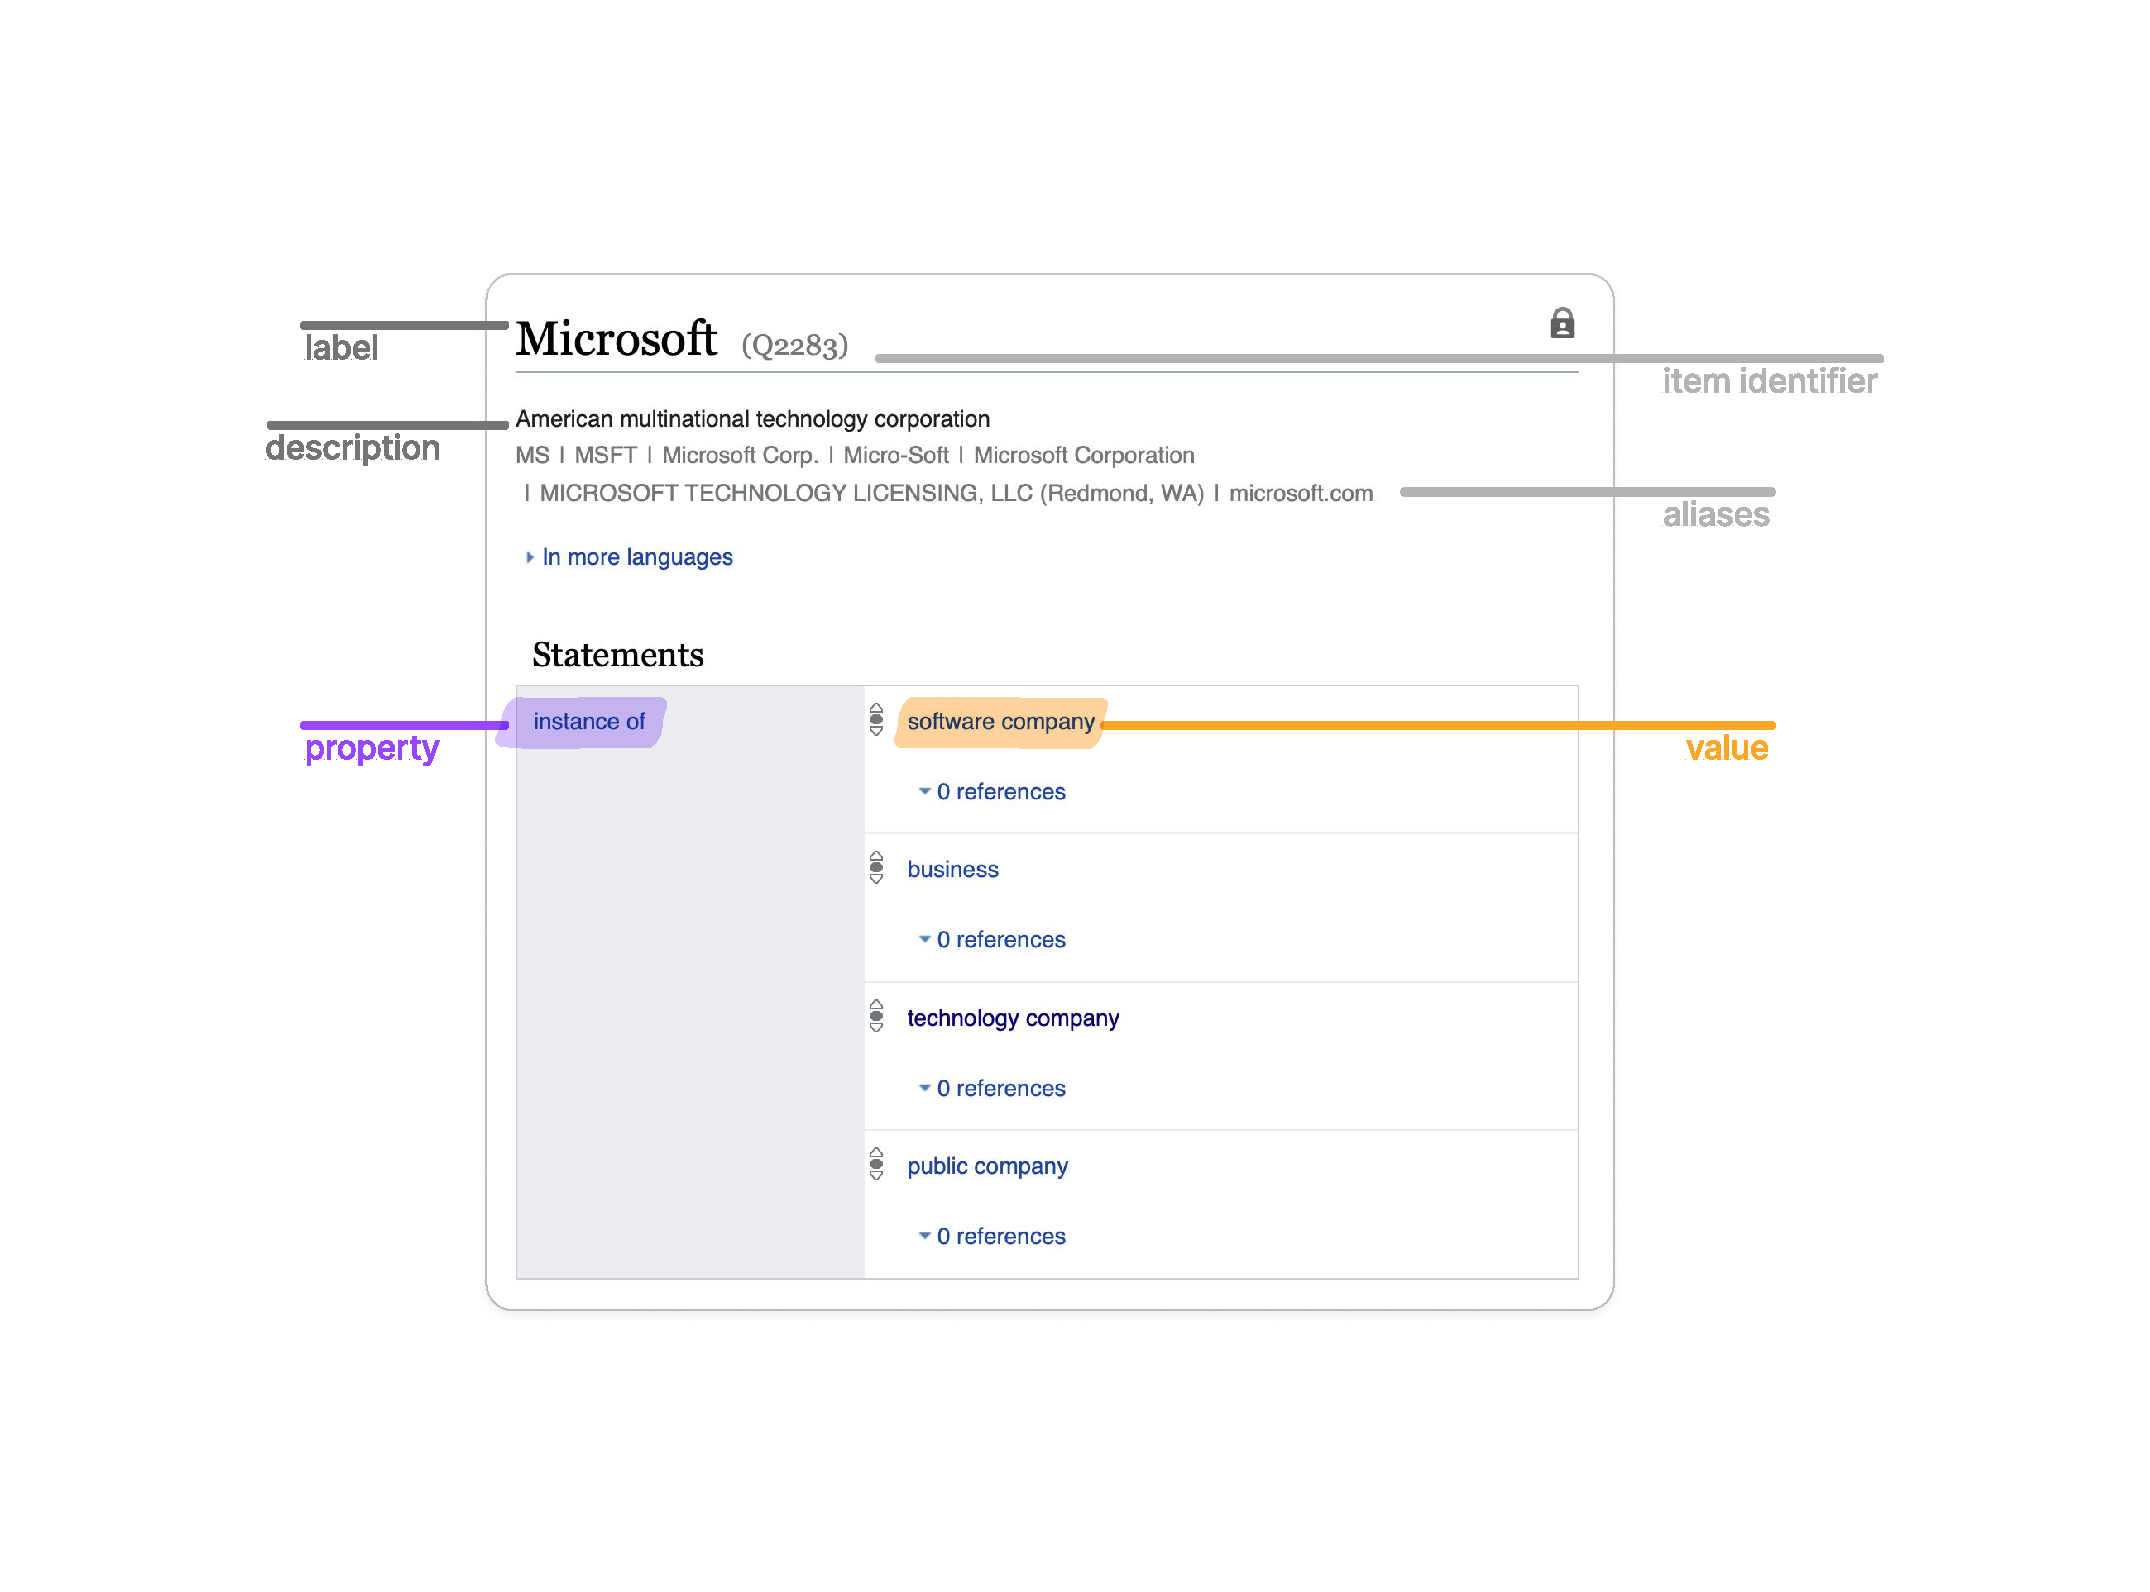
\includegraphics[width=\textwidth]{img/wikidata-microsoft.pdf}
    \caption{Wikidata item for Microsoft.}
    \label{fig:wikidata-microsoft}
\end{figure}

Wikidata consists of items with unique identifiers, denoted as Q<number> as QID. In Figure \ref{fig:wikidata-microsoft}, the identifier for the item labelled as Microsoft is Q2283. This item has the description ``\textit{American multinational technology corporation}'' and several aliases (also known as). Items in Wikidata provide statements containing individual properties tagged P<number> and their corresponding values. These values can have various types, including multiple values, item values, quantitative values, and unknown or no values. Microsoft has a property \textit{instance of}, which refers to multiple item values describing Microsoft as a software company, enterprise, technology company, and public company. In this case, the individual values refer to other items. Additional information can be found in Wikidata glossary \parencite{wikidata_glossary}.

\subsection{Spacy Entity Linker}
\label{subsec:spacy-entity-linker}
The most suitable solution for our problem, which meets the requirements and provides adequate integration with our spaCy implementation of the named entity recognition module, is the Spacy Entity Linker library in Python, available on GitHub\footnote{\href{https://www.github.com/egerber/spaCy-entity-linker}{https://www.github.com/egerber/spaCy-entity-linker}}. This library creates a pipeline with an external knowledge base built on Wikidata that matches possible entities from the text with potential entities (the Entity Linker refers to each item in Wikidata as an entity) on Wikidata. The main advantage of this library is that each entity found in the text provides a QID on Wikidata, allowing us to obtain additional information about the entity, including its label, aliases, description, and more.

The main priority now is to filter out entities in the text that are not identified as organizations. The Entity Linker does not provide entity type information to determine if an entity is an organization. Instead, it only uses references to other entities via the properties \textit{instance of} (P31), \textit{part of} (P361) and eventually \textit{subclass of} (P279) to determine the type. For example, when we extract the entity Microsoft, we obtain information about the categories (understood as types) it belongs to, such as software company, business, technology company, and public company, which can further branch into various subcategories. This allows an entity to be part of a wide range of possible classes. However, even if an entity belongs to the organization class according to our criteria, it may be labelled differently and miss one of the classes, causing us to lose the extracted entity. Therefore, we stick to the original partitioning associated with the organization type that handles the initial named entity recognition and compare it with the entities extracted from the entity linker using span. Additionally, staying with the original implementation of spaCy entity objects in the code will make our work more manageable in the next phase of sentiment analysis and encourage code consistency.

The Entity Linker only uses the properties we mentioned when categorizing into classes. Thus, we can not directly get information about the ticker using the Entity Linker since the \textit{stock exchange} property provides the ticker information. Regardless of aliases, it would be necessary to compare them with a database of tickers to see if one of the many aliases has an exact match. However, the Entity Linker provides us with the QID of the entity, which we can use to get any information about the entity. This opens up several possibilities for us to get this data. First, we tried the pywikibot\footnote{\href{https://www.github.com/wikimedia/pywikibot}{https://www.github.com/wikimedia/pywikibot}} library, which works similarly to scraping. This approach is not ideal, as each entity page must first be created as an object and then loaded from the page repository, where the data is extracted. However, it is much more efficient and more accessible to query Wikidata using the Wikidata SPARQL endpoint, giving us more modularity and flexibility we want to maintain in the code.

\subsection{SPARQL Wrapper}
\label{subsubsec:sparql-wrapper}
Access to Wikidata's SPARQL endpoint is enabled by the SPARQL Wrapper library in Python, which is available on GitHub\footnote{\href{https://www.github.com/egerber/spaCy-entity-linker/tree/master}{https://www.github.com/egerber/spaCy-entity-linker/tree/master}}. Now, we have a tool that we can use to query data about entities with a given QID using SPARQL. We will show three queries that cover the most common situations where we want to get a ticker along with the name of the exchange on which the company is traded. The queries are run sequentially, with each subsequent query processing entity that did not produce a result in the previous query\todo{QA: Dlouho jsem hledal nějakou operaci jak sekvenční přístup nahradit a všechny queries sloučit do jedné. Nakonec se mi ale líbí, navíc můžeme přidávat další filtry za sebe.}. We also mention the list of essential properties that we will use in the queries:

\begin{itemize}
    \item \textbf{P414}: The \textbf{\textit{stock exchange}} on which the entity is traded.
    \item \textbf{P249}: The \textbf{\textit{ticker symbol}} of the entity.
    \item \textbf{P582}: The \textbf{\textit{end time}} of the property.
    \item \textbf{P127}: The entity \textbf{\textit{owned by}} by another entity.
    \item \textbf{P1889}: The entity is \textbf{\textit{different from}} another entity.
\end{itemize}

To better illustrate, we add an Instagram entity to the actual entities extracted from our sample Guardian article to demonstrate the second query associated with the \textit{owned by} property. The reader can try the following queries on the Wikidata SPARQL endpoint{\footnote{\href{https://www.query.wikidata.org/}{https://www.query.wikidata.org/}}.

\subsubsection{Query 1: Direct ticker retrieval}
\label{subsubsec:q1-direct-ticker-retrieval}
The first query aims to retrieve information about a \textit{ticker symbol} and a \textit{stock exchange} associated with an entity's \textit{stock exchange} property. The SPARQL query can be found in Appendix \ref{appsec:q1-direct-ticker-retrieval}. This query selects entities that directly possess the \textit{stock exchange} property, providing details about the ticker symbols and the exchanges on which the entities are traded. It also filters the results to include only those records where the exchanges do not have an \textit{end time} specified. The results of this query are presented in Table \ref{table:sparql_query_1_results}.

\begin{table}[ht]
    \centering
    \caption{The results of the SPARQL Query 1: Direct ticker retrieval.}
    \label{table:sparql_query_1_results}
    \begin{tabular}{l l l l}
    \hline
    \multicolumn{2}{c}{Organisation} & \multirow{2}{*}{Ticker} & \multirow{2}{*}{Stock Exchange}\\
    \cline{1-2}
    QID & Label \\
    \hline
    Q11463 & Adobe & ADBE & NASDAQ \\ 
    Q3884 & Amazon & AMZN & NASDAQ \\ 
    Q37156 & IBM & IBM & NYSE \\ 
    Q2283 & Microsoft & MSFT & NASDAQ \\
    \hline
    \end{tabular}
\end{table}

The data retrieved for individual organizations is accurate. Nevertheless, the results do not include the expected information about the Google entity. Although Google has a ticker through the \textit{stock exchange} property on Wikidata, it also has an \textit{end time} value set despite still being tradable on NASDAQ under the tickers GOOG and GOOGL.\todo{QA/TODO: Dodat, že není tolik běžné, že mají companies na námi specializoavných burzách více než 2 tickery a pro jednoduchost aplikace a struktury od každé entity vezmeme pouze jeden. Na druhou stranu jsem ještě nikdy neviděl API, které by zahrnovalo více než jeden ticker na company, protože mi přijde, že se od jednoho dají další odvodit. Pro jednoduchost a implementační záležitosti zatím volím raději pro jeden ticker. Co si o tom myslíte Vy?} At the time of writing, this \textit{end time} value can not be edited for unknown reasons, which presents a limitation we must accept. Consequently, additional queries are needed to determine details for the entities Meta, TikTok, OpenAI, and Instagram.

\subsubsection{Query 2: Owner-based ticker retrieval}
\label{subsubsec:q2-owner-based-ticker-retrieval}

The second query focuses on retrieving information about the exchange and ticker of the entities associated with the querying entity through an \textit{owned by} relationship. The SPARQL query is displayed in Appendix \ref{appsec:q2-owner-based-ticker-retrieval}. This query selects entities with the \textit{owned by} property and retrieves information about the tickers and exchanges associated with those entities. It explicitly targets entities related to the queried entity through the \textit{owned by} property. The results of this query are shown in Table \ref{table:sparql_query_2_results}.

\begin{table}[ht]
    \centering
    \caption{The results of the SPARQL Query 2: Owner-based ticker retrieval.}
    \label{table:sparql_query_2_results}
    \begin{tabular}{l l l l}
    \hline
    \multicolumn{2}{c}{Organisation} & \multirow{2}{*}{Ticker} & \multirow{2}{*}{Stock Exchange}\\
    \cline{1-2}
    QID & Label \\
    \hline
    Q209330 & Instagram & META & NASDAQ \\ \hline
    \end{tabular}
\end{table}

The retrieved data are again accurate. Meta Platforms indeed own Instagram, which is accessed through the Instagram \textit{owned by} Meta Platforms association. In this case, we successfully filtered out the FB ticker, now META\footnote{\href{https://www.bloomberg.com/quote/FB:US}{https://www.bloomberg.com/quote/FB:US}}, due to the \textit{end time} filtering.

\subsubsection{Query 3: Differentiated ticker retrieval}
\label{subsubsec:q3-differentiated-ticker-retrieval}
The third query retrieves information about the exchange and ticker of entities associated with the querying entity through a \textit{different from} relationship. The SPARQL query is presented in Appendix \ref{appsec:q3-differentiated-ticker-retrieval}. Similar to the owner-based ticker retrieval, this query selects entities with the \textit{different from} property and retrieves information about the tickers and exchanges associated with those entities. It focuses on entities related to the queried entity through the \textit{different from} property. The results of this query are shown in Table \ref{table:sparql_query_3_results}.

\begin{table}[ht]
    \centering
    \caption{The results of the SPARQL Query 3: Differentiated ticker retrieval.}
    \label{table:sparql_query_3_results}
    \begin{tabular}{l l l l}
    \hline
    \multicolumn{2}{c}{Organisation} & \multirow{2}{*}{Ticker} & \multirow{2}{*}{Stock Exchange}\\
    \cline{1-2}
    QID & Label \\
    \hline
    Q18811574 & Meta & META & NASDAQ \\ \hline
    \end{tabular}
\end{table}    

Again, the obtained data aligns with what is generally accepted as accurate. However, it is essential to note that Meta represents multiple distinct entities (as many others) on Wikidata. Therefore, querying the \textit{different from} property is necessary in this context to retrieve Meta Platforms.

\subsubsection*{Summary}
\label{subsubsec:sparql-wrapper-summary}
Using the three queries outlined above, we have successfully covered a noteworthy amount of organizations that are directly traded or have relationships with companies traded on the exchange. As shown in Table \ref{table:sparql-all-queries-results}, we achieved an almost one hundred per cent success rate. However, Google is not included in the results due to the previously mentioned issue with the \textit{end time} setting. We must accept this limitation for now and will not alter our overall approach because of one entity. Regarding changing the data in Wikidata, a future opportunity to modify can arise.

Additionally, TikTok and OpenAI are absent in the results, which is expected since neither has a ticker or a relationship with a company traded on an exchange. Our querying approach allows flexibility, enabling us to create additional filtering queries as needed. This flexibility is a valuable advantage in refining our results.

\begin{table}[ht]
    \centering
    \caption{The results of the SPARQL queries for all extracted organisation names from the Guardian's article.}
    \label{table:sparql-all-queries-results}
    \begin{tabular}{l l l l}
    \hline
    \multicolumn{2}{c}{Organisation} & \multirow{2}{*}{Ticker} & \multirow{2}{*}{Stock Exchange}\\
    \cline{1-2}
    QID & Label \\
    \hline
    Q11463 & Adobe & ADBE & NASDAQ \\ 
    Q3884 & Amazon & AMZN & NASDAQ \\ 
    Q37156 & IBM & IBM & NYSE \\ 
    Q2283 & Microsoft & MSFT & NASDAQ \\
    Q209330 & Instagram & META & NASDAQ \\   
    Q18811574 & Meta & META & NASDAQ \\ 
    \hline
    \end{tabular}
\end{table} 